\chapter{Kletterroboter}
\section{Motivation}
Die meisten abgegebenen Aufgaben des Workshops sind sehr programmierlastig. Konstruktionen treten oftmals gegenüber den Programmen in den Hintergrund darum fiel die Wahl für den zweiten Workshop auf eine Konstruktionsaufgaben, den Kletterroboter 


\section{Geschichte}
Ein Erdbeben erschüttert die Stadt! In einem Hochhaus sind durch ein Erdbeben die Treppen eingestürzt. Lediglich der Fahrstuhlschacht ist noch intakt. Der Roboter muss den Menschen zur Hilfe eilen in dem er den Fahrstuhlschacht hoch klettert.

\begin{capfigure}[Kletterroboter]
	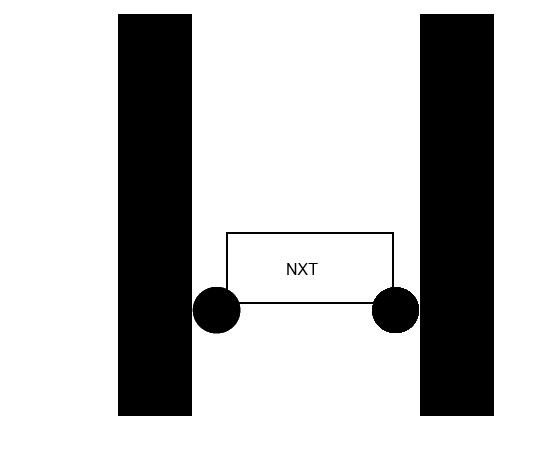
\includegraphics[width=10cm]{images/klettern_skizze}
\end{capfigure}

\section{Aufgabenstellung}
Bauen Sie einen Roboter der zwischen zwei senkrecht aufgestellten. Tischen aus eigener kraft bis zu einer Höhe von 70cm hoch- und auf 50cm runter fahren kann, ohne abzurutschen. Es sind nur die Bauteile aus dem Standardbaukasten erlaubt. Die Abstandsmessung soll mit dem Ultraschallsensor erfolgen. 
    
\section{Lösung}
wie anfangs erwähnt, besteht der größte Teil der Lösung in der Konstruktion des Kletterroboters.
    
\subsection{Konstruktion}
Der Standardbaukasten enthält nur eine sehr begrenzte Anzahl an Getriebe Elementen, keine Bänder oder Ketten und wenige ausladende Trägerelemente. Zudem ist der Steuerbaustein des NXT Moduls aufgrund der Akkus sehr schwer, was eine Erschwernis bezüglich der Anforderungen der Konstruktion darstellt, bezüglich des Antriebs und der aufzubringenden Reibung darstellt.
      
Anleitungen für einen Kletterer erfüllten verschiedene Kriterien, wie der Standardbaukasten nicht und konnten nicht verwendet werden. Darum wurde eine exklusive Eigenkonstruktion entwickelt.
Die Anforderungen stellen sich wie folgt zusammen:
      
\begin{itemize}
	\item möglichst wenige Bauteile
	\item geringe Bauhöhe für schmalen Schacht,
	\item optimale Raumausnutzung
	\item gute Positionierung des Ultraschallsensors zum Boden
	\item automatisches Festklemmen an den Wänden
	\item einfache Bedienbarkeit des NXT Steins im Schacht
\end{itemize}
      
Zusätzlich kommen folgende Schwierigkeiten hinzu:
      
\begin{itemize}
	\item hohes Gewicht der Bauteile
	\item nur Teile von Standardbaukasten
	\item begrenzte Kraft der Motoren von Akkus
\end{itemize}

Die Antwort auf die o.g. Probleme besteht, wie von den Bildern zu entnehmen ist, aus einem modular aufgebauten Roboter, der aus dem Klemmer, der Antriebsmotoren und der NXT Stein besteht. Die Module sind nur jeweils mit 2 Stiften mit einander verbunden und lassen sich so schnell auseinander nehmen.
      
\begin{capfigure}[Kletterroboter Profil links]
	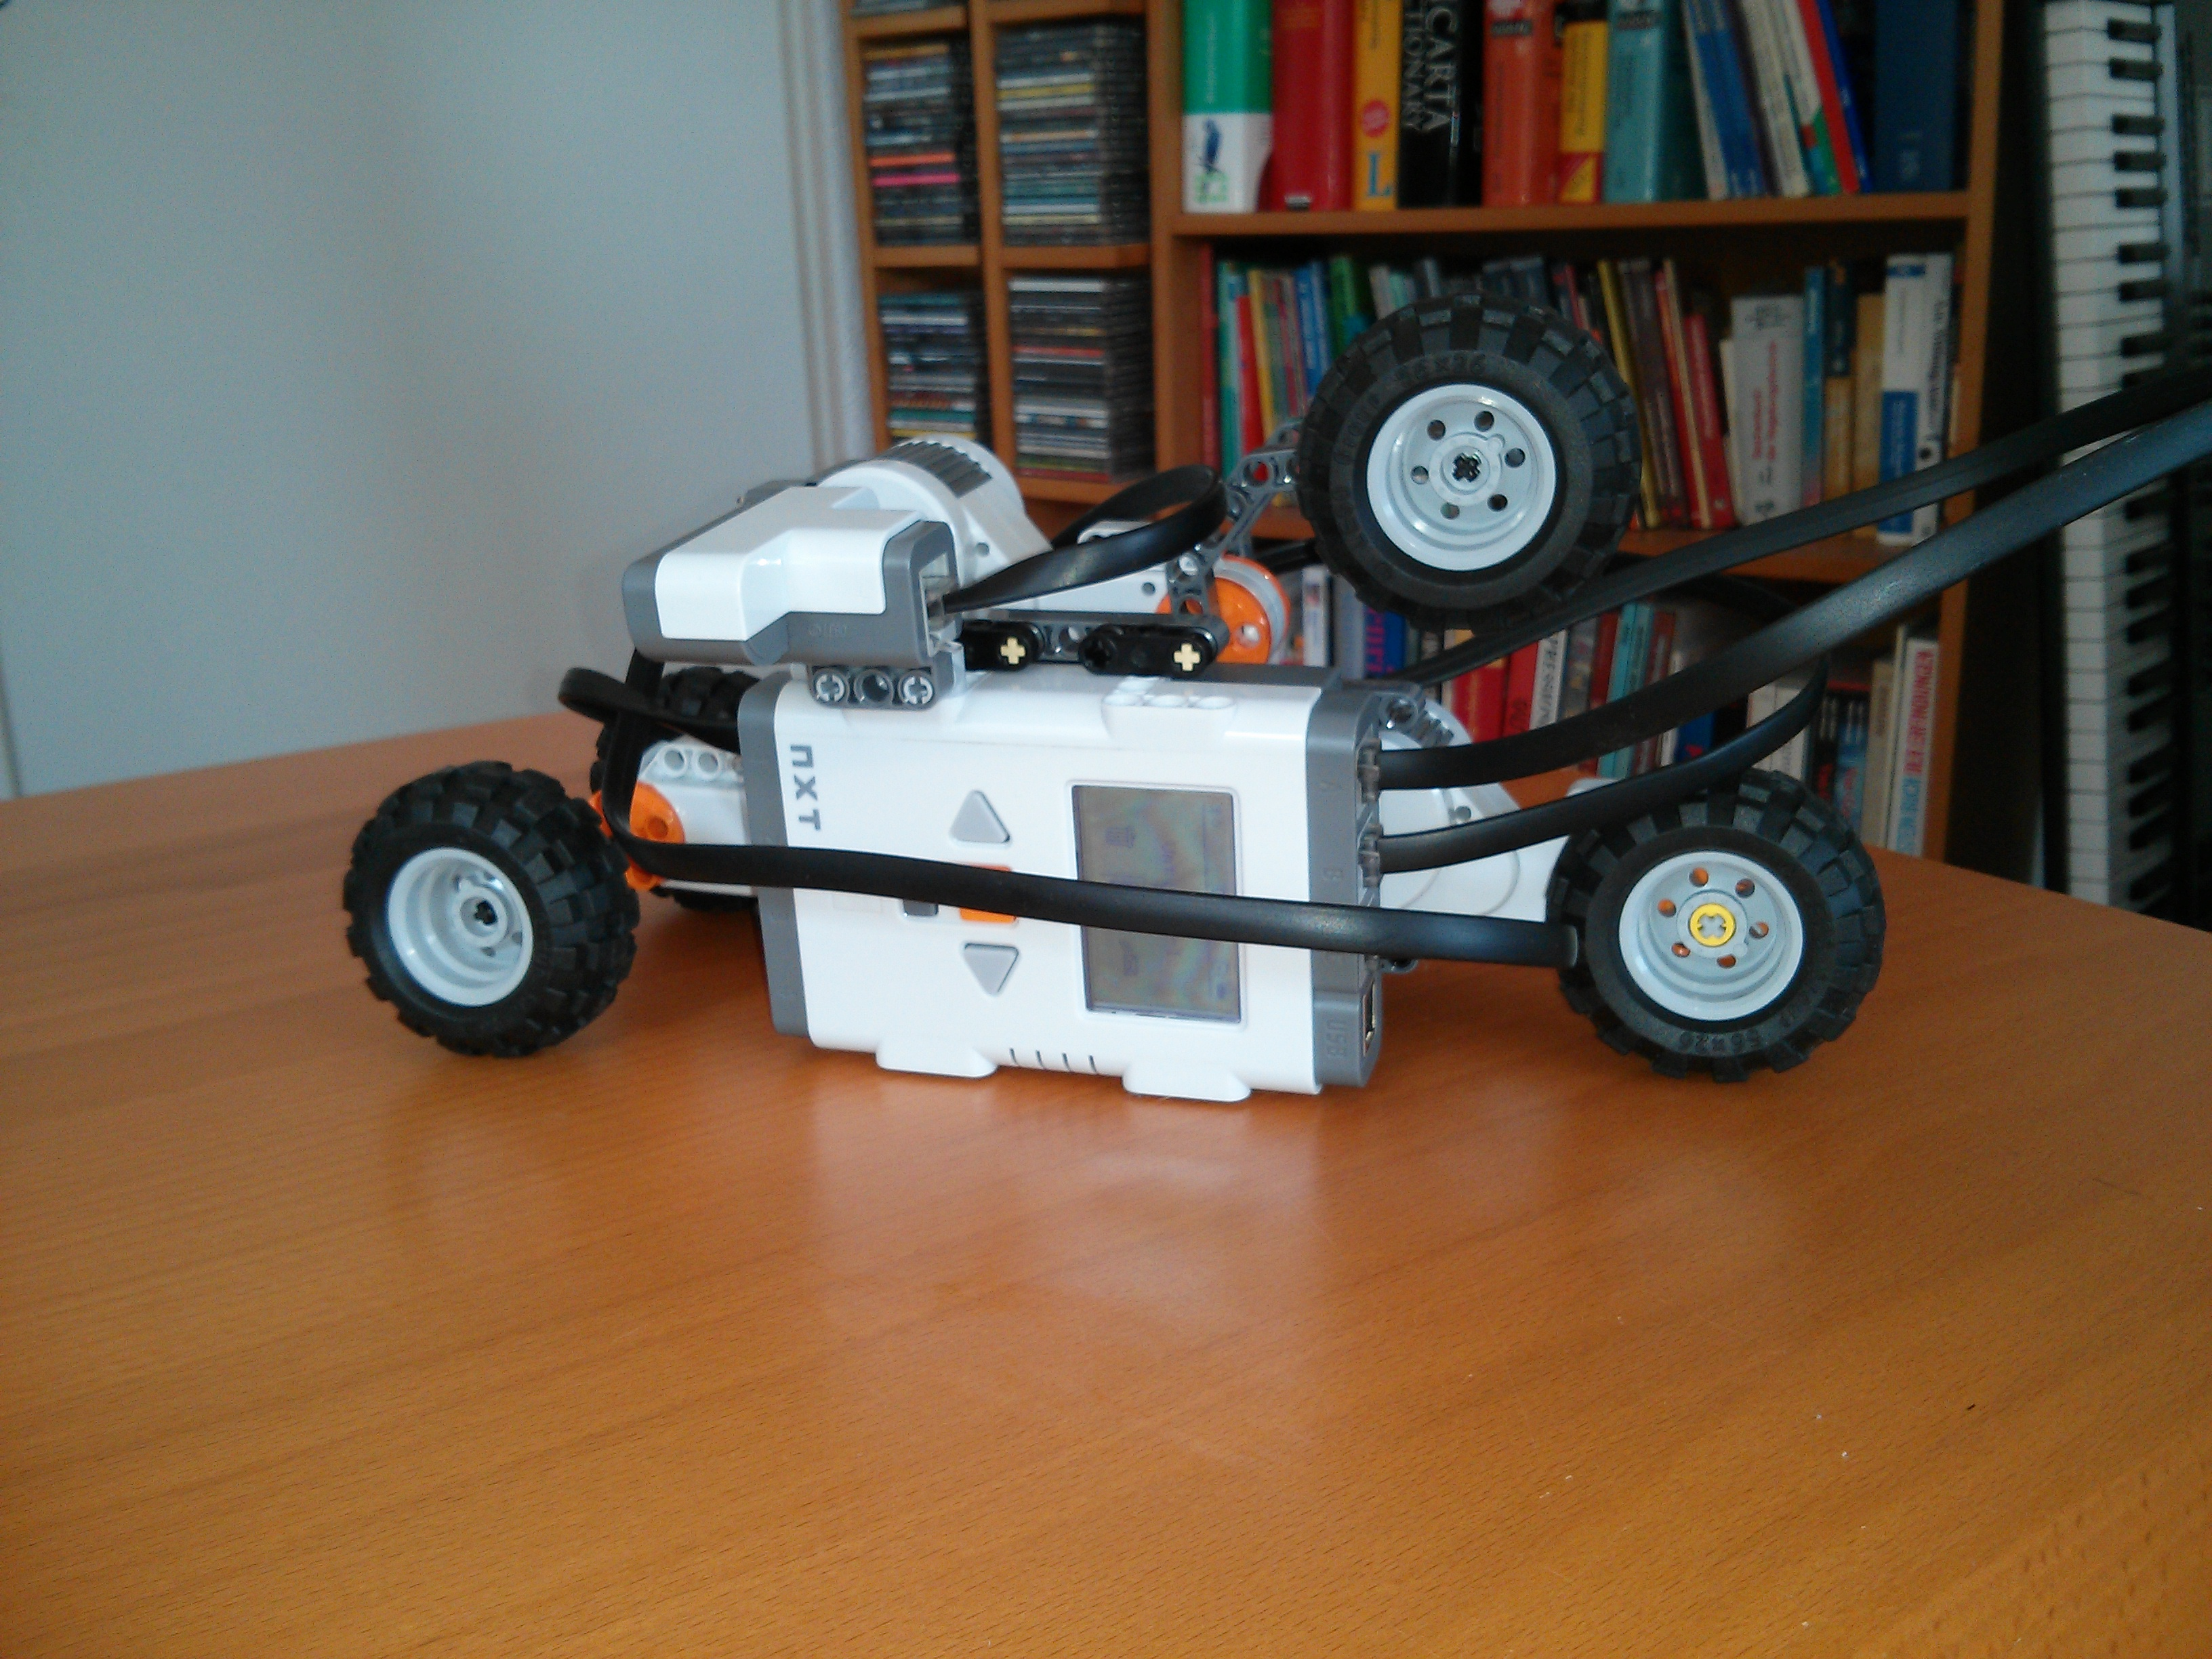
\includegraphics[width=10cm]{images/kletter1.jpg}
\end{capfigure}
      
Aus Platzmangel und von der Gewichtsvereilung her war es nicht möglich, die Motoren unter den NXT Bautein anzuorden. Die Bedienbarkeit hätte ebenfalls gelitten. Darum wurde der Stein einfach seitlich um 90 gedreht angebracht. Auf der einen Seite befinden sich also die 3 Motoren auf der anderen der Baustein. Somit ist das Gefährt ausbalanciert. Da die Anzahl an Reifen auf 4 Begrenzt ist, wurde vorn auf ein Rad verzichtet und ein Rad mittig angeordnet. Zusammen mit der unteren beiden Rädern wird ein Verwinkeln und ein Kursabweichen vermieden, um den Roboter gerade nach oben zu führen. 
            
\begin{capfigure}[Kletterroboter Profil rechts]
	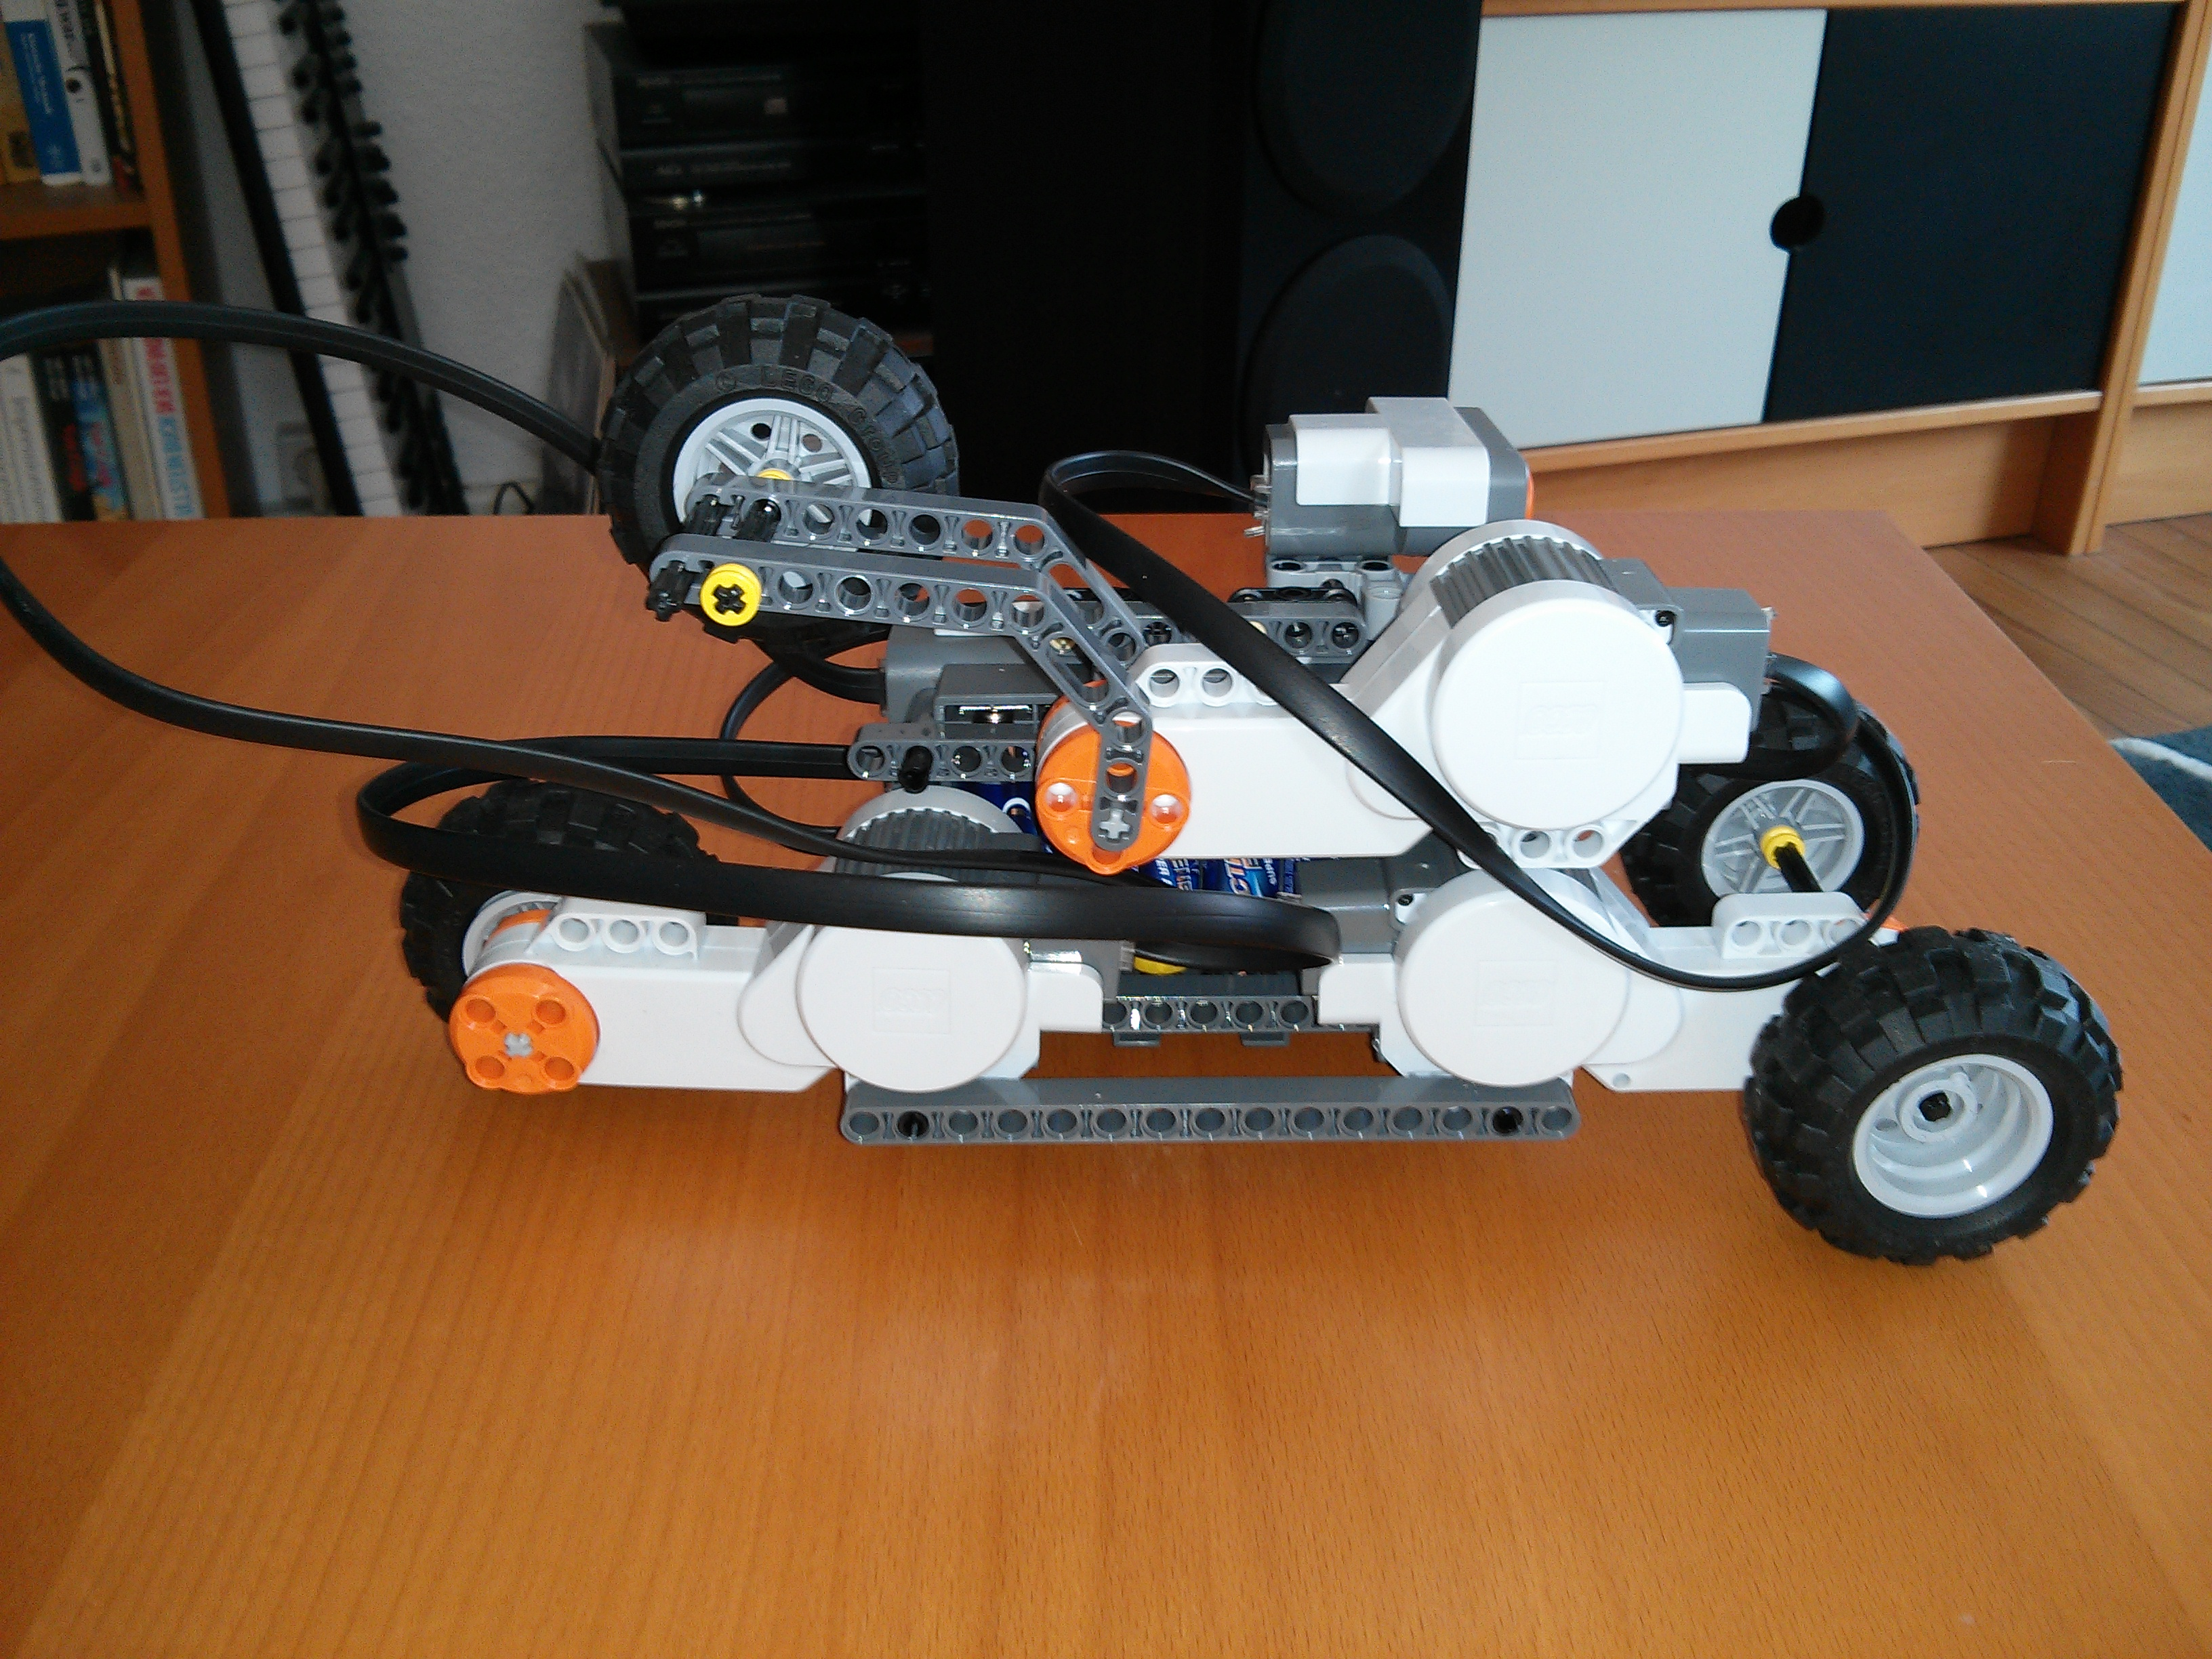
\includegraphics[width=10cm]{images/kletter2.jpg}
\end{capfigure}
      
Das Klemmrad bildet zusammen mit den Antriebsrädern ebenfalls ein Kräftedreieck. Es ist so aufgebaut, dass es etwa nach einem Drittel der Fahrzeuglänge ansetzt. Es entsteht wieder ein Kräftedreieck. Der Allradantrieb sorgt, schafft gegenüber des entstehenden Moments, welches zusätzlichen Druck auf das Klemmrad ausüben könnte Abhilfe. Versuche ohne die Allradkonstruktion führten zu einem Nachgeben der Klemme und damit zum Absturz.
      
\begin{capfigure}[Kletterroboter Profil rechts]
	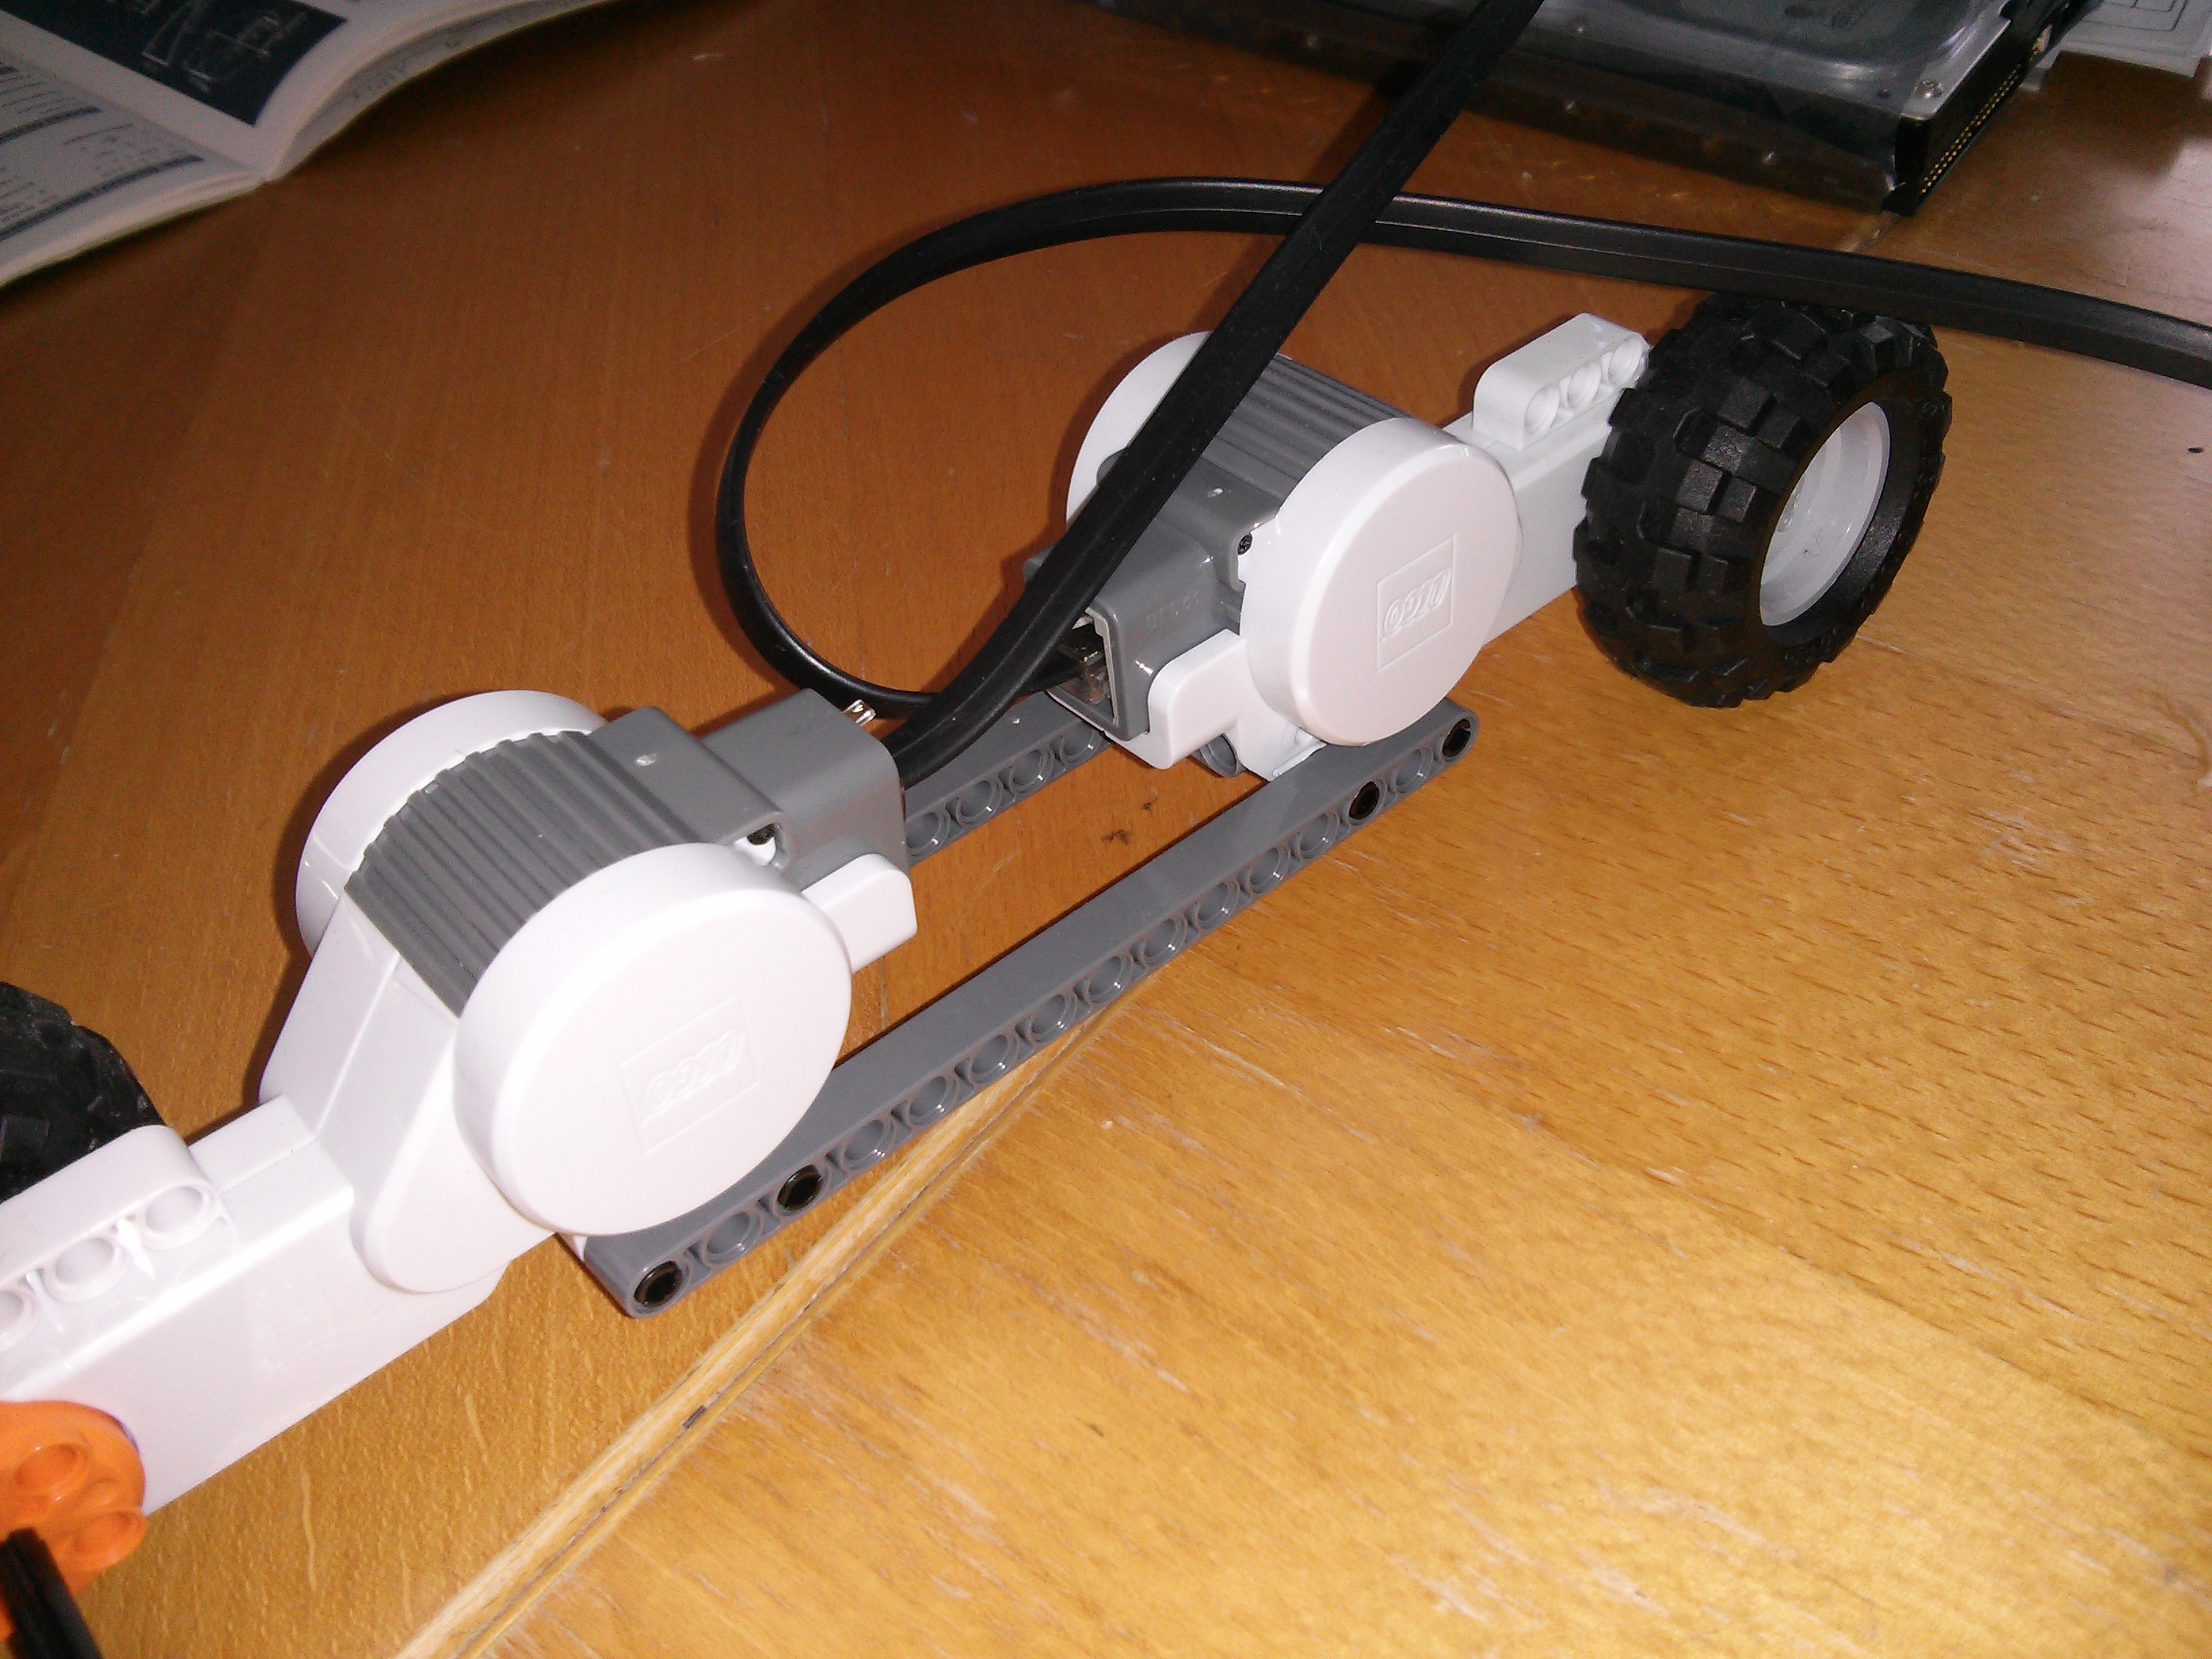
\includegraphics[width=10cm]{images/kletter3.jpg}
\end{capfigure}
    
Auf dem NXT Stein ist der Ultraschallsensor mit Blick nach unten angebracht. Er ist bewusst nicht so weit unten platziert, damit der Sensor schon in Bodennähe zuverlässige Daten liefern kann. Er liefert nämlich erst ab etwa 20cm Abstand zuverlässige 
    
\subsection{Code}
Der Code des Kletterroboters ist ein Einzeiler, der die Motoren in Bewegung setzt und diese blockiert, sobald der Sensor ein paar mal hintereinander den einen Wert, der Größer als eine Schranke ist. 
    
Die Lösung liegt auf der DVD unter \textit{Lösungen/Kletterer}. 